
\chapter{Modbus Secure}
\label{secure}

The Modbus Secure protocol uses the same frames as the TCP
standard encapsulated through a TLS channel.
The TLS protocol provides an authentication system using x.509v3 certificates. 
The Modbus Secure standard requires
TLS with version 1.2 or higher (we are currently at version 1.3),
the client supports both versions (1.2 and 1.3). 
The use of certificates requires the creation of a certificate and a
private key for the server (slave), as well as for 
each client that will connect to the server (slave). 
A diagram is given below to clarify the
roles of both server-side and client-side certificates:

\begin{figure}[H]
  \centering
  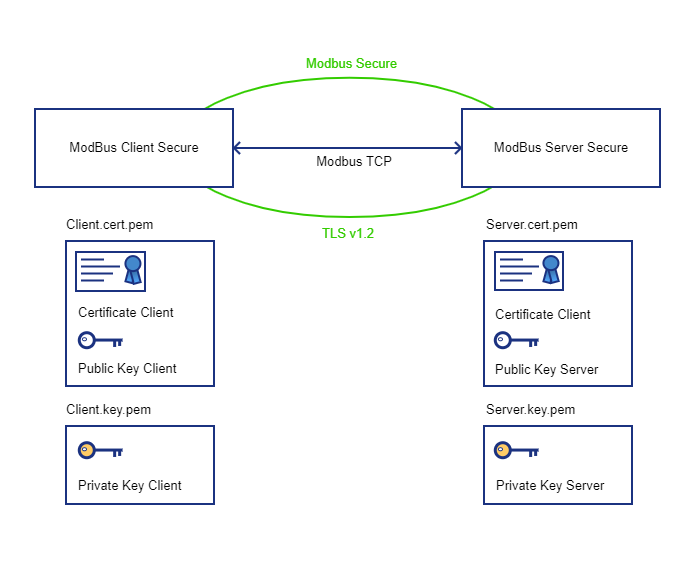
\includegraphics[width=0.8\textwidth]{../Img/schemamodbussecure.png}
  \caption{Modbus Secure certificate scheme}
\end{figure}

The standard requires certain extensions to be added to the x.509v3 certificate including an OID (Object
Identifier standardized by the International Telecomunications Union) to define the role of the client at the
time of authentication. In fact, the specification stipulates that all clients can use read functions
read functions but only clients with the role of "operator" can use write functions (of coils or holding
registers).

\newpage
\section{Modbus Secure Specification}

The main specifications of the MB-TCP\_Security-v21\_2018-07-24 regulations are given below:

\begin{itemize}
    \item The protocol version must be $\ge$ TLS 1.2
    \item Cipher suite: RSA for key exchange
    \item Cipher suite: AES128 for packet encryption
    \item Cipher suite: SHA256SUM for the integrity check of the messages
    \item Default cipher: TLS\_RSA\_WITH\_AES\_128\_CBC\_SHA256
\end{itemize}

\section{X509v3 extensions}

The following are the contents of the extensions that the standard requires 
to be added to a standard X509v3 certificate:

\begin{verbatim}
X509v3 extensions:
  X509v3 Subject Key Identifier:
      38:A4:CC:19:6D:6D:E2:AA:7C:82:75:44:A0:59:39:81:47:D3:13:F0
  X509v3 Authority Key Identifier:
      keyid:38:A4:CC:19:6D:6D:E2:AA:7C:82:75:44:A0:59:39:81:47:D3:13:F0

  X509v3 Basic Constraints:
      CA:FALSE
  X509v3 Key Usage: critical
      Digital Signature, Non Repudiation, Key Encipherment
  1.3.6.1.4.1.50316.802.1:
      ..Operator
  X509v3 Subject Alternative Name:
      IP Address:192.168.1.10
\end{verbatim}

\newpage
\section{Certificate generation}

The steps to generate certificates with openssl are as follows (multiple rows are handled so the 
commands can be copied and pasted directly to the shell console):
\\\\
Generate certificate and private key for the server (change the ip to the correct server address):

\begin{verbatim}
# Server
  openssl req -x509 -newkey rsa:4096 -sha256 -days 360 \
  -keyout server.key.pem -out server.cert.pem \
  -nodes -subj "/C=IT/ST=Italy/L=Rovereto/O=ModBusServer/OU=ModBusServer/CN=ModbusSecurityServer" \
  -addext "keyUsage=critical,digitalSignature,nonRepudiation,keyEncipherment" \
  -addext "subjectAltName=IP:192.168.1.20"
\end{verbatim}

Generate one or more certificates/private keys for the clients that 
will connect to the server (three examples are given below, 
as before the ip address must be updated with the correct one):

\begin{verbatim}
# Client 1:
  openssl req -x509 -newkey rsa:4096 -sha256 -days 360 \
  -keyout client1.key.pem -out client1.cert.pem -nodes \
  -subj "/C=IT/ST=Italy/L=Rovereto/O=ModBusClient/OU=ModBusClient/CN=ModbusSecurityClient" \
  -addext "keyUsage=critical,digitalSignature,nonRepudiation,keyEncipherment" \
  -addext "1.3.6.1.4.1.50316.802.1=ASN1:UTF8String:Operator" \
  -addext "subjectAltName=IP:192.168.1.10"
\end{verbatim}

On some operating-systems very often the certificate+private key pair is merged into a 
single password-protected file (.pfx).
To merge certificate and key into a single pfx file use the following command:

\begin{verbatim}
  openssl pkcs12 -export -out client1.pfx -inkey client1.key.pem -in client1.cert.pem
\end{verbatim}

To view the content of a certificate use the following command:

\begin{verbatim}
  openssl x509 -in client1.cert.pem -text
\end{verbatim}
